\documentclass[1p]{elsarticle_modified}
%\bibliographystyle{elsarticle-num}

%\usepackage[colorlinks]{hyperref}
%\usepackage{abbrmath_seonhwa} %\Abb, \Ascr, \Acal ,\Abf, \Afrak
\usepackage{amsfonts}
\usepackage{amssymb}
\usepackage{amsmath}
\usepackage{amsthm}
\usepackage{scalefnt}
\usepackage{amsbsy}
\usepackage{kotex}
\usepackage{caption}
\usepackage{subfig}
\usepackage{color}
\usepackage{graphicx}
\usepackage{xcolor} %% white, black, red, green, blue, cyan, magenta, yellow
\usepackage{float}
\usepackage{setspace}
\usepackage{hyperref}

\usepackage{tikz}
\usetikzlibrary{arrows}

\usepackage{multirow}
\usepackage{array} % fixed length table
\usepackage{hhline}

%%%%%%%%%%%%%%%%%%%%%
\makeatletter
\renewcommand*\env@matrix[1][\arraystretch]{%
	\edef\arraystretch{#1}%
	\hskip -\arraycolsep
	\let\@ifnextchar\new@ifnextchar
	\array{*\c@MaxMatrixCols c}}
\makeatother %https://tex.stackexchange.com/questions/14071/how-can-i-increase-the-line-spacing-in-a-matrix
%%%%%%%%%%%%%%%

\usepackage[normalem]{ulem}

\newcommand{\msout}[1]{\ifmmode\text{\sout{\ensuremath{#1}}}\else\sout{#1}\fi}
%SOURCE: \msout is \stkout macro in https://tex.stackexchange.com/questions/20609/strikeout-in-math-mode

\newcommand{\cancel}[1]{
	\ifmmode
	{\color{red}\msout{#1}}
	\else
	{\color{red}\sout{#1}}
	\fi
}

\newcommand{\add}[1]{
	{\color{blue}\uwave{#1}}
}

\newcommand{\replace}[2]{
	\ifmmode
	{\color{red}\msout{#1}}{\color{blue}\uwave{#2}}
	\else
	{\color{red}\sout{#1}}{\color{blue}\uwave{#2}}
	\fi
}

\newcommand{\Sol}{\mathcal{S}} %segment
\newcommand{\D}{D} %diagram
\newcommand{\A}{\mathcal{A}} %arc


%%%%%%%%%%%%%%%%%%%%%%%%%%%%%5 test

\def\sl{\operatorname{\textup{SL}}(2,\Cbb)}
\def\psl{\operatorname{\textup{PSL}}(2,\Cbb)}
\def\quan{\mkern 1mu \triangleright \mkern 1mu}

\theoremstyle{definition}
\newtheorem{thm}{Theorem}[section]
\newtheorem{prop}[thm]{Proposition}
\newtheorem{lem}[thm]{Lemma}
\newtheorem{ques}[thm]{Question}
\newtheorem{cor}[thm]{Corollary}
\newtheorem{defn}[thm]{Definition}
\newtheorem{exam}[thm]{Example}
\newtheorem{rmk}[thm]{Remark}
\newtheorem{alg}[thm]{Algorithm}

\newcommand{\I}{\sqrt{-1}}
\begin{document}

%\begin{frontmatter}
%
%\title{Boundary parabolic representations of knots up to 8 crossings}
%
%%% Group authors per affiliation:
%\author{Yunhi Cho} 
%\address{Department of Mathematics, University of Seoul, Seoul, Korea}
%\ead{yhcho@uos.ac.kr}
%
%
%\author{Seonhwa Kim} %\fnref{s_kim}}
%\address{Center for Geometry and Physics, Institute for Basic Science, Pohang, 37673, Korea}
%\ead{ryeona17@ibs.re.kr}
%
%\author{Hyuk Kim}
%\address{Department of Mathematical Sciences, Seoul National University, Seoul 08826, Korea}
%\ead{hyukkim@snu.ac.kr}
%
%\author{Seokbeom Yoon}
%\address{Department of Mathematical Sciences, Seoul National University, Seoul, 08826,  Korea}
%\ead{sbyoon15@snu.ac.kr}
%
%\begin{abstract}
%We find all boundary parabolic representation of knots up to 8 crossings.
%
%\end{abstract}
%\begin{keyword}
%    \MSC[2010] 57M25 
%\end{keyword}
%
%\end{frontmatter}

%\linenumbers
%\tableofcontents
%
\newcommand\colored[1]{\textcolor{white}{\rule[-0.35ex]{0.8em}{1.4ex}}\kern-0.8em\color{red} #1}%
%\newcommand\colored[1]{\textcolor{white}{ #1}\kern-2.17ex	\textcolor{white}{ #1}\kern-1.81ex	\textcolor{white}{ #1}\kern-2.15ex\color{red}#1	}

{\Large $\underline{12a_{0809}~(K12a_{0809})}$}

\setlength{\tabcolsep}{10pt}
\renewcommand{\arraystretch}{1.6}
\vspace{1cm}\begin{tabular}{m{100pt}>{\centering\arraybackslash}m{274pt}}
\multirow{5}{120pt}{
	\centering
	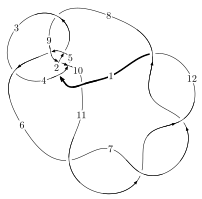
\includegraphics[width=112pt]{../../../GIT/diagram.site/Diagrams/png/1610_12a_0809.png}\\
\ \ \ A knot diagram\footnotemark}&
\allowdisplaybreaks
\textbf{Linearized knot diagam} \\
\cline{2-2}
 &
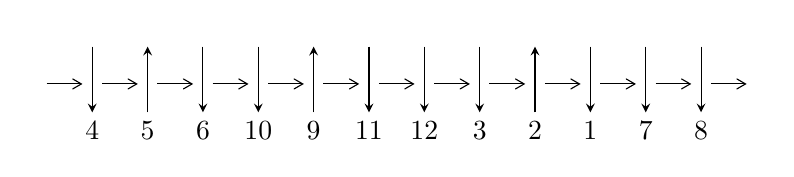
\begin{tikzpicture}[x=20pt, y=17pt]
	% nodes
	\node (C0) at (0, 0) {};
	\node (C1) at (1, 0) {};
	\node (C1U) at (1, +1) {};
	\node (C1D) at (1, -1) {4};

	\node (C2) at (2, 0) {};
	\node (C2U) at (2, +1) {};
	\node (C2D) at (2, -1) {5};

	\node (C3) at (3, 0) {};
	\node (C3U) at (3, +1) {};
	\node (C3D) at (3, -1) {6};

	\node (C4) at (4, 0) {};
	\node (C4U) at (4, +1) {};
	\node (C4D) at (4, -1) {10};

	\node (C5) at (5, 0) {};
	\node (C5U) at (5, +1) {};
	\node (C5D) at (5, -1) {9};

	\node (C6) at (6, 0) {};
	\node (C6U) at (6, +1) {};
	\node (C6D) at (6, -1) {11};

	\node (C7) at (7, 0) {};
	\node (C7U) at (7, +1) {};
	\node (C7D) at (7, -1) {12};

	\node (C8) at (8, 0) {};
	\node (C8U) at (8, +1) {};
	\node (C8D) at (8, -1) {3};

	\node (C9) at (9, 0) {};
	\node (C9U) at (9, +1) {};
	\node (C9D) at (9, -1) {2};

	\node (C10) at (10, 0) {};
	\node (C10U) at (10, +1) {};
	\node (C10D) at (10, -1) {1};

	\node (C11) at (11, 0) {};
	\node (C11U) at (11, +1) {};
	\node (C11D) at (11, -1) {7};

	\node (C12) at (12, 0) {};
	\node (C12U) at (12, +1) {};
	\node (C12D) at (12, -1) {8};
	\node (C13) at (13, 0) {};

	% arrows
	\draw[->,>={angle 60}]
	(C0) edge (C1) (C1) edge (C2) (C2) edge (C3) (C3) edge (C4) (C4) edge (C5) (C5) edge (C6) (C6) edge (C7) (C7) edge (C8) (C8) edge (C9) (C9) edge (C10) (C10) edge (C11) (C11) edge (C12) (C12) edge (C13) ;	\draw[->,>=stealth]
	(C1U) edge (C1D) (C2D) edge (C2U) (C3U) edge (C3D) (C4U) edge (C4D) (C5D) edge (C5U) (C6U) edge (C6D) (C7U) edge (C7D) (C8U) edge (C8D) (C9D) edge (C9U) (C10U) edge (C10D) (C11U) edge (C11D) (C12U) edge (C12D) ;
	\end{tikzpicture} \\
\hhline{~~} \\& 
\textbf{Solving Sequence} \\ \cline{2-2} 
 &
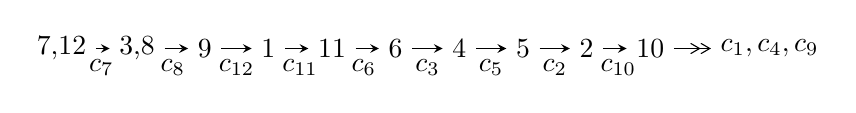
\begin{tikzpicture}[x=23pt, y=7pt]
	% node
	\node (A0) at (-1/8, 0) {7,12};
	\node (A1) at (17/16, 0) {3,8};
	\node (A2) at (17/8, 0) {9};
	\node (A3) at (25/8, 0) {1};
	\node (A4) at (33/8, 0) {11};
	\node (A5) at (41/8, 0) {6};
	\node (A6) at (49/8, 0) {4};
	\node (A7) at (57/8, 0) {5};
	\node (A8) at (65/8, 0) {2};
	\node (A9) at (73/8, 0) {10};
	\node (C1) at (1/2, -1) {$c_{7}$};
	\node (C2) at (13/8, -1) {$c_{8}$};
	\node (C3) at (21/8, -1) {$c_{12}$};
	\node (C4) at (29/8, -1) {$c_{11}$};
	\node (C5) at (37/8, -1) {$c_{6}$};
	\node (C6) at (45/8, -1) {$c_{3}$};
	\node (C7) at (53/8, -1) {$c_{5}$};
	\node (C8) at (61/8, -1) {$c_{2}$};
	\node (C9) at (69/8, -1) {$c_{10}$};
	\node (A10) at (11, 0) {$c_{1},c_{4},c_{9}$};

	% edge
	\draw[->,>=stealth]	
	(A0) edge (A1) (A1) edge (A2) (A2) edge (A3) (A3) edge (A4) (A4) edge (A5) (A5) edge (A6) (A6) edge (A7) (A7) edge (A8) (A8) edge (A9) ;
	\draw[->>,>={angle 60}]	
	(A9) edge (A10);
\end{tikzpicture} \\ 

\end{tabular} \\

\footnotetext{
The image of knot diagram is generated by the software ``\textbf{Draw programme}" developed by Andrew Bartholomew(\url{http://www.layer8.co.uk/maths/draw/index.htm\#Running-draw}), where we modified some parts for our purpose(\url{https://github.com/CATsTAILs/LinksPainter}).
}\phantom \\ \newline 
\centering \textbf{Ideals for irreducible components\footnotemark of $X_{\text{par}}$} 
 
\begin{align*}
I^u_{1}&=\langle 
148539 u^{48}-527493 u^{47}+\cdots+8051 b-394683,\;95347 u^{48}-282451 u^{47}+\cdots+32204 a+36495,\\
\phantom{I^u_{1}}&\phantom{= \langle  }u^{49}-5 u^{48}+\cdots+17 u+4\rangle \\
I^u_{2}&=\langle 
2517 u^{34} a+42256 u^{34}+\cdots+6152 a+31050,\;6 u^{34} a-3 u^{34}+\cdots+6 a-17,\;u^{35}+2 u^{34}+\cdots+4 u-1\rangle \\
I^u_{3}&=\langle 
u^{12}+u^{11}-6 u^{10}-6 u^9+12 u^8+13 u^7-9 u^6-12 u^5+2 u^4+4 u^3+u^2+b+u+1,\\
\phantom{I^u_{3}}&\phantom{= \langle  }- u^{14}+u^{13}+8 u^{12}-7 u^{11}-23 u^{10}+17 u^9+28 u^8-16 u^7-13 u^6+5 u^5+u^4-3 u^3+3 u^2+a+2 u+1,\\
\phantom{I^u_{3}}&\phantom{= \langle  }u^{15}-2 u^{14}-7 u^{13}+15 u^{12}+17 u^{11}-40 u^{10}-18 u^9+45 u^8+14 u^7-22 u^6-13 u^5+8 u^4+u^3+u^2+1\rangle \\
I^u_{4}&=\langle 
a u+b+u+1,\;a^2+3 a u+2 a+u+4,\;u^2+u-1\rangle \\
\\
\end{align*}
\raggedright * 4 irreducible components of $\dim_{\mathbb{C}}=0$, with total 138 representations.\\
\footnotetext{All coefficients of polynomials are rational numbers. But the coefficients are sometimes approximated in decimal forms when there is not enough margin.}
\newpage
\renewcommand{\arraystretch}{1}
\centering \section*{I. $I^u_{1}= \langle 148539 u^{48}-527493 u^{47}+\cdots+8051 b-394683,\;95347 u^{48}-282451 u^{47}+\cdots+32204 a+36495,\;u^{49}-5 u^{48}+\cdots+17 u+4 \rangle$}
\flushleft \textbf{(i) Arc colorings}\\
\begin{tabular}{m{7pt} m{180pt} m{7pt} m{180pt} }
\flushright $a_{7}=$&$\begin{pmatrix}1\\0\end{pmatrix}$ \\
\flushright $a_{12}=$&$\begin{pmatrix}0\\u\end{pmatrix}$ \\
\flushright $a_{3}=$&$\begin{pmatrix}-2.96072 u^{48}+8.77068 u^{47}+\cdots-24.7516 u-1.13324\\-18.4498 u^{48}+65.5189 u^{47}+\cdots+241.353 u+49.0229\end{pmatrix}$ \\
\flushright $a_{8}=$&$\begin{pmatrix}1\\u^2\end{pmatrix}$ \\
\flushright $a_{9}=$&$\begin{pmatrix}-7.08294 u^{48}+17.6739 u^{47}+\cdots+1.25894 u+5.64181\\-27.2013 u^{48}+89.0489 u^{47}+\cdots+287.738 u+59.6427\end{pmatrix}$ \\
\flushright $a_{1}=$&$\begin{pmatrix}- u\\- u^3+u\end{pmatrix}$ \\
\flushright $a_{11}=$&$\begin{pmatrix}u\\u\end{pmatrix}$ \\
\flushright $a_{6}=$&$\begin{pmatrix}- u^2+1\\- u^2\end{pmatrix}$ \\
\flushright $a_{4}=$&$\begin{pmatrix}-4.22094 u^{48}+9.52301 u^{47}+\cdots-21.4049 u+0.492516\\-11.5817 u^{48}+33.6645 u^{47}+\cdots+72.2484 u+16.8837\end{pmatrix}$ \\
\flushright $a_{5}=$&$\begin{pmatrix}-8.39172 u^{48}+25.3461 u^{47}+\cdots+57.0803 u+14.9414\\-12.9692 u^{48}+37.3577 u^{47}+\cdots+90.6477 u+20.3169\end{pmatrix}$ \\
\flushright $a_{2}=$&$\begin{pmatrix}4.12132 u^{48}-18.5185 u^{47}+\cdots-157.649 u-27.2511\\2.08806 u^{48}-10.1386 u^{47}+\cdots-96.3135 u-16.4853\end{pmatrix}$ \\
\flushright $a_{10}=$&$\begin{pmatrix}- u^5+2 u^3+u\\- u^7+3 u^5-2 u^3+u\end{pmatrix}$\\&\end{tabular}
\flushleft \textbf{(ii) Obstruction class $= -1$}\\~\\
\flushleft \textbf{(iii) Cusp Shapes $= \frac{1218}{83} u^{48}-\frac{2750}{83} u^{47}+\cdots+\frac{7009}{83} u-\frac{594}{83}$}\\~\\
\newpage\renewcommand{\arraystretch}{1}
\flushleft \textbf{(iv) u-Polynomials at the component}\newline \\
\begin{tabular}{m{50pt}|m{274pt}}
Crossings & \hspace{64pt}u-Polynomials at each crossing \\
\hline $$\begin{aligned}c_{1},c_{3}\end{aligned}$$&$\begin{aligned}
&u^{49}+8 u^{48}+\cdots+17 u-1
\end{aligned}$\\
\hline $$\begin{aligned}c_{2}\end{aligned}$$&$\begin{aligned}
&u^{49}+26 u^{48}+\cdots+11 u+2
\end{aligned}$\\
\hline $$\begin{aligned}c_{4},c_{8}\end{aligned}$$&$\begin{aligned}
&u^{49}+5 u^{47}+\cdots+3 u+1
\end{aligned}$\\
\hline $$\begin{aligned}c_{5},c_{9}\end{aligned}$$&$\begin{aligned}
&u^{49}- u^{48}+\cdots+27 u^2+1
\end{aligned}$\\
\hline $$\begin{aligned}c_{6},c_{7},c_{11}\\c_{12}\end{aligned}$$&$\begin{aligned}
&u^{49}-5 u^{48}+\cdots+17 u+4
\end{aligned}$\\
\hline $$\begin{aligned}c_{10}\end{aligned}$$&$\begin{aligned}
&u^{49}-9 u^{48}+\cdots-1017 u+2272
\end{aligned}$\\
\hline
\end{tabular}\\~\\
\newpage\renewcommand{\arraystretch}{1}
\flushleft \textbf{(v) Riley Polynomials at the component}\newline \\
\begin{tabular}{m{50pt}|m{274pt}}
Crossings & \hspace{64pt}Riley Polynomials at each crossing \\
\hline $$\begin{aligned}c_{1},c_{3}\end{aligned}$$&$\begin{aligned}
&y^{49}-22 y^{48}+\cdots+199 y-1
\end{aligned}$\\
\hline $$\begin{aligned}c_{2}\end{aligned}$$&$\begin{aligned}
&y^{49}+20 y^{47}+\cdots+89 y-4
\end{aligned}$\\
\hline $$\begin{aligned}c_{4},c_{8}\end{aligned}$$&$\begin{aligned}
&y^{49}+10 y^{48}+\cdots-9 y-1
\end{aligned}$\\
\hline $$\begin{aligned}c_{5},c_{9}\end{aligned}$$&$\begin{aligned}
&y^{49}+25 y^{48}+\cdots-54 y-1
\end{aligned}$\\
\hline $$\begin{aligned}c_{6},c_{7},c_{11}\\c_{12}\end{aligned}$$&$\begin{aligned}
&y^{49}-55 y^{48}+\cdots+137 y-16
\end{aligned}$\\
\hline $$\begin{aligned}c_{10}\end{aligned}$$&$\begin{aligned}
&y^{49}+9 y^{48}+\cdots-108326159 y-5161984
\end{aligned}$\\
\hline
\end{tabular}\\~\\
\newpage\flushleft \textbf{(vi) Complex Volumes and Cusp Shapes}
$$\begin{array}{c|c|c}  
\text{Solutions to }I^u_{1}& \I (\text{vol} + \sqrt{-1}CS) & \text{Cusp shape}\\
 \hline 
\begin{aligned}
u &= -0.860395 + 0.482404 I \\
a &= \phantom{-}0.024941 + 0.522248 I \\
b &= -0.236258 + 0.004668 I\end{aligned}
 & -1.333090 - 0.442268 I & -22.7302 - 2.7893 I \\ \hline\begin{aligned}
u &= -0.860395 - 0.482404 I \\
a &= \phantom{-}0.024941 - 0.522248 I \\
b &= -0.236258 - 0.004668 I\end{aligned}
 & -1.333090 + 0.442268 I & -22.7302 + 2.7893 I \\ \hline\begin{aligned}
u &= \phantom{-}1.038190 + 0.218664 I \\
a &= \phantom{-}0.962395 + 0.159463 I \\
b &= \phantom{-}0.063672 - 0.241113 I\end{aligned}
 & -3.12377 - 8.13177 I & \phantom{-0.000000 -}0. + 9.34743 I \\ \hline\begin{aligned}
u &= \phantom{-}1.038190 - 0.218664 I \\
a &= \phantom{-}0.962395 - 0.159463 I \\
b &= \phantom{-}0.063672 + 0.241113 I\end{aligned}
 & -3.12377 + 8.13177 I & \phantom{-0.000000 } 0. - 9.34743 I \\ \hline\begin{aligned}
u &= -0.656302 + 0.593975 I \\
a &= \phantom{-}1.73077 + 1.26119 I \\
b &= \phantom{-}0.157164 + 0.032896 I\end{aligned}
 & \phantom{-}1.0974 + 15.3120 I & -6.69862 - 10.70010 I \\ \hline\begin{aligned}
u &= -0.656302 - 0.593975 I \\
a &= \phantom{-}1.73077 - 1.26119 I \\
b &= \phantom{-}0.157164 - 0.032896 I\end{aligned}
 & \phantom{-}1.0974 - 15.3120 I & -6.69862 + 10.70010 I \\ \hline\begin{aligned}
u &= -0.527749 + 0.624204 I \\
a &= -0.344437 - 0.796756 I \\
b &= -0.374375 + 0.028886 I\end{aligned}
 & -0.22239 + 2.13464 I & -12.97767 - 4.41434 I \\ \hline\begin{aligned}
u &= -0.527749 - 0.624204 I \\
a &= -0.344437 + 0.796756 I \\
b &= -0.374375 - 0.028886 I\end{aligned}
 & -0.22239 - 2.13464 I & -12.97767 + 4.41434 I \\ \hline\begin{aligned}
u &= -0.598351 + 0.535692 I \\
a &= -1.55845 - 1.25421 I \\
b &= \phantom{-}0.013056 + 0.352563 I\end{aligned}
 & -0.78788 + 6.56431 I & -12.9454 - 9.8564 I \\ \hline\begin{aligned}
u &= -0.598351 - 0.535692 I \\
a &= -1.55845 + 1.25421 I \\
b &= \phantom{-}0.013056 - 0.352563 I\end{aligned}
 & -0.78788 - 6.56431 I & -12.9454 + 9.8564 I\\
 \hline 
 \end{array}$$\newpage$$\begin{array}{c|c|c}  
\text{Solutions to }I^u_{1}& \I (\text{vol} + \sqrt{-1}CS) & \text{Cusp shape}\\
 \hline 
\begin{aligned}
u &= -0.747144\phantom{ +0.000000I} \\
a &= \phantom{-}0.385007\phantom{ +0.000000I} \\
b &= -0.305862\phantom{ +0.000000I}\end{aligned}
 & -1.10744\phantom{ +0.000000I} & -7.81270\phantom{ +0.000000I} \\ \hline\begin{aligned}
u &= -0.162177 + 0.729155 I \\
a &= \phantom{-}0.300367 - 0.459004 I \\
b &= \phantom{-}0.409646 - 0.408558 I\end{aligned}
 & \phantom{-}0.80721 + 4.71794 I & -9.1417 - 13.3340 I \\ \hline\begin{aligned}
u &= -0.162177 - 0.729155 I \\
a &= \phantom{-}0.300367 + 0.459004 I \\
b &= \phantom{-}0.409646 + 0.408558 I\end{aligned}
 & \phantom{-}0.80721 - 4.71794 I & -9.1417 + 13.3340 I \\ \hline\begin{aligned}
u &= \phantom{-}0.744466 + 0.003975 I \\
a &= -1.81736 + 0.85970 I \\
b &= -0.328629 + 0.159289 I\end{aligned}
 & -4.13096 + 1.69814 I & -18.2040 - 4.3712 I \\ \hline\begin{aligned}
u &= \phantom{-}0.744466 - 0.003975 I \\
a &= -1.81736 - 0.85970 I \\
b &= -0.328629 - 0.159289 I\end{aligned}
 & -4.13096 - 1.69814 I & -18.2040 + 4.3712 I \\ \hline\begin{aligned}
u &= -0.300631 + 0.671867 I \\
a &= \phantom{-}0.481511 + 0.645526 I \\
b &= \phantom{-}0.987848 + 0.795214 I\end{aligned}
 & \phantom{-}2.15150 - 11.04750 I & -4.44153 + 5.63378 I \\ \hline\begin{aligned}
u &= -0.300631 - 0.671867 I \\
a &= \phantom{-}0.481511 - 0.645526 I \\
b &= \phantom{-}0.987848 - 0.795214 I\end{aligned}
 & \phantom{-}2.15150 + 11.04750 I & -4.44153 - 5.63378 I \\ \hline\begin{aligned}
u &= \phantom{-}0.485135 + 0.542391 I \\
a &= \phantom{-}0.943805 - 0.987006 I \\
b &= \phantom{-}0.402923 - 0.436742 I\end{aligned}
 & \phantom{-}2.90214 - 1.87444 I & -0.73211 + 3.66192 I \\ \hline\begin{aligned}
u &= \phantom{-}0.485135 - 0.542391 I \\
a &= \phantom{-}0.943805 + 0.987006 I \\
b &= \phantom{-}0.402923 + 0.436742 I\end{aligned}
 & \phantom{-}2.90214 + 1.87444 I & -0.73211 - 3.66192 I \\ \hline\begin{aligned}
u &= \phantom{-}1.289650 + 0.140107 I \\
a &= \phantom{-}0.300793 - 0.515547 I \\
b &= -0.125058 + 0.334394 I\end{aligned}
 & -2.81136 + 8.04498 I & \phantom{-0.000000 } 0\\
 \hline 
 \end{array}$$\newpage$$\begin{array}{c|c|c}  
\text{Solutions to }I^u_{1}& \I (\text{vol} + \sqrt{-1}CS) & \text{Cusp shape}\\
 \hline 
\begin{aligned}
u &= \phantom{-}1.289650 - 0.140107 I \\
a &= \phantom{-}0.300793 + 0.515547 I \\
b &= -0.125058 - 0.334394 I\end{aligned}
 & -2.81136 - 8.04498 I & \phantom{-0.000000 } 0 \\ \hline\begin{aligned}
u &= \phantom{-}0.506307 + 0.409416 I \\
a &= -2.22196 + 1.72599 I \\
b &= -0.776269 + 0.644378 I\end{aligned}
 & -1.37259 - 1.45940 I & -10.10356 + 4.62979 I \\ \hline\begin{aligned}
u &= \phantom{-}0.506307 - 0.409416 I \\
a &= -2.22196 - 1.72599 I \\
b &= -0.776269 - 0.644378 I\end{aligned}
 & -1.37259 + 1.45940 I & -10.10356 - 4.62979 I \\ \hline\begin{aligned}
u &= -0.340049 + 0.552838 I \\
a &= \phantom{-}0.176095 - 0.121875 I \\
b &= -0.914800 - 0.629603 I\end{aligned}
 & -0.03939 - 2.80450 I & -9.90854 + 3.00975 I \\ \hline\begin{aligned}
u &= -0.340049 - 0.552838 I \\
a &= \phantom{-}0.176095 + 0.121875 I \\
b &= -0.914800 + 0.629603 I\end{aligned}
 & -0.03939 + 2.80450 I & -9.90854 - 3.00975 I \\ \hline\begin{aligned}
u &= -0.537786 + 0.350030 I \\
a &= -0.059222 - 1.272190 I \\
b &= \phantom{-}0.103070 + 0.635374 I\end{aligned}
 & -1.62694 + 1.54828 I & -11.08710 - 6.22827 I \\ \hline\begin{aligned}
u &= -0.537786 - 0.350030 I \\
a &= -0.059222 + 1.272190 I \\
b &= \phantom{-}0.103070 - 0.635374 I\end{aligned}
 & -1.62694 - 1.54828 I & -11.08710 + 6.22827 I \\ \hline\begin{aligned}
u &= \phantom{-}1.47621 + 0.08489 I \\
a &= -0.950241 + 0.354999 I \\
b &= -1.43618 - 0.18131 I\end{aligned}
 & -5.81539 + 0.81969 I & \phantom{-0.000000 } 0 \\ \hline\begin{aligned}
u &= \phantom{-}1.47621 - 0.08489 I \\
a &= -0.950241 - 0.354999 I \\
b &= -1.43618 + 0.18131 I\end{aligned}
 & -5.81539 - 0.81969 I & \phantom{-0.000000 } 0 \\ \hline\begin{aligned}
u &= -1.52067 + 0.14417 I \\
a &= -0.937215 - 0.026137 I \\
b &= -1.98715 - 0.67865 I\end{aligned}
 & -3.73933 + 4.27877 I & \phantom{-0.000000 } 0\\
 \hline 
 \end{array}$$\newpage$$\begin{array}{c|c|c}  
\text{Solutions to }I^u_{1}& \I (\text{vol} + \sqrt{-1}CS) & \text{Cusp shape}\\
 \hline 
\begin{aligned}
u &= -1.52067 - 0.14417 I \\
a &= -0.937215 + 0.026137 I \\
b &= -1.98715 + 0.67865 I\end{aligned}
 & -3.73933 - 4.27877 I & \phantom{-0.000000 } 0 \\ \hline\begin{aligned}
u &= -1.55060 + 0.10978 I \\
a &= \phantom{-}1.84193 - 0.18622 I \\
b &= \phantom{-}4.05332 + 0.45056 I\end{aligned}
 & -8.35293 + 3.28009 I & \phantom{-0.000000 } 0 \\ \hline\begin{aligned}
u &= -1.55060 - 0.10978 I \\
a &= \phantom{-}1.84193 + 0.18622 I \\
b &= \phantom{-}4.05332 - 0.45056 I\end{aligned}
 & -8.35293 - 3.28009 I & \phantom{-0.000000 } 0 \\ \hline\begin{aligned}
u &= \phantom{-}1.54635 + 0.18703 I \\
a &= \phantom{-}0.757838 - 0.546719 I \\
b &= \phantom{-}1.80903 - 1.20397 I\end{aligned}
 & -7.12280 - 5.06000 I & \phantom{-0.000000 } 0 \\ \hline\begin{aligned}
u &= \phantom{-}1.54635 - 0.18703 I \\
a &= \phantom{-}0.757838 + 0.546719 I \\
b &= \phantom{-}1.80903 + 1.20397 I\end{aligned}
 & -7.12280 + 5.06000 I & \phantom{-0.000000 } 0 \\ \hline\begin{aligned}
u &= \phantom{-}1.55747 + 0.09309 I \\
a &= \phantom{-}0.98887 - 1.45323 I \\
b &= \phantom{-}2.04164 - 2.22854 I\end{aligned}
 & -8.74919 - 3.11091 I & \phantom{-0.000000 } 0 \\ \hline\begin{aligned}
u &= \phantom{-}1.55747 - 0.09309 I \\
a &= \phantom{-}0.98887 + 1.45323 I \\
b &= \phantom{-}2.04164 + 2.22854 I\end{aligned}
 & -8.74919 + 3.11091 I & \phantom{-0.000000 } 0 \\ \hline\begin{aligned}
u &= \phantom{-}1.56503 + 0.15811 I \\
a &= \phantom{-}2.12720 - 0.54206 I \\
b &= \phantom{-}4.43010 - 0.79741 I\end{aligned}
 & -8.03789 - 9.09579 I & \phantom{-0.000000 } 0 \\ \hline\begin{aligned}
u &= \phantom{-}1.56503 - 0.15811 I \\
a &= \phantom{-}2.12720 + 0.54206 I \\
b &= \phantom{-}4.43010 + 0.79741 I\end{aligned}
 & -8.03789 + 9.09579 I & \phantom{-0.000000 } 0 \\ \hline\begin{aligned}
u &= -1.59257 + 0.00650 I \\
a &= \phantom{-}1.97070 + 0.65045 I \\
b &= \phantom{-}4.19761 + 1.43756 I\end{aligned}
 & -12.06900 - 1.62283 I & \phantom{-0.000000 } 0\\
 \hline 
 \end{array}$$\newpage$$\begin{array}{c|c|c}  
\text{Solutions to }I^u_{1}& \I (\text{vol} + \sqrt{-1}CS) & \text{Cusp shape}\\
 \hline 
\begin{aligned}
u &= -1.59257 - 0.00650 I \\
a &= \phantom{-}1.97070 - 0.65045 I \\
b &= \phantom{-}4.19761 - 1.43756 I\end{aligned}
 & -12.06900 + 1.62283 I & \phantom{-0.000000 } 0 \\ \hline\begin{aligned}
u &= \phantom{-}1.58602 + 0.18202 I \\
a &= -2.19854 + 0.10847 I \\
b &= -4.50456 + 0.32567 I\end{aligned}
 & -6.4148 - 18.1914 I & \phantom{-0.000000 } 0 \\ \hline\begin{aligned}
u &= \phantom{-}1.58602 - 0.18202 I \\
a &= -2.19854 - 0.10847 I \\
b &= -4.50456 - 0.32567 I\end{aligned}
 & -6.4148 + 18.1914 I & \phantom{-0.000000 } 0 \\ \hline\begin{aligned}
u &= -0.240166 + 0.320881 I \\
a &= \phantom{-}0.947458 + 0.195457 I \\
b &= -0.450401 + 0.404469 I\end{aligned}
 & -0.963675 + 0.866301 I & -7.31478 - 5.07695 I \\ \hline\begin{aligned}
u &= -0.240166 - 0.320881 I \\
a &= \phantom{-}0.947458 - 0.195457 I \\
b &= -0.450401 - 0.404469 I\end{aligned}
 & -0.963675 - 0.866301 I & -7.31478 + 5.07695 I \\ \hline\begin{aligned}
u &= \phantom{-}1.61021 + 0.11898 I \\
a &= -1.070280 + 0.513665 I \\
b &= -1.94637 + 0.86375 I\end{aligned}
 & -9.61044 - 1.58418 I & \phantom{-0.000000 } 0 \\ \hline\begin{aligned}
u &= \phantom{-}1.61021 - 0.11898 I \\
a &= -1.070280 - 0.513665 I \\
b &= -1.94637 - 0.86375 I\end{aligned}
 & -9.61044 + 1.58418 I & \phantom{-0.000000 } 0 \\ \hline\begin{aligned}
u &= -1.64403 + 0.02832 I \\
a &= -1.71447 + 0.78931 I \\
b &= -3.43609 + 1.41784 I\end{aligned}
 & -12.1970 + 8.7921 I & \phantom{-0.000000 } 0 \\ \hline\begin{aligned}
u &= -1.64403 - 0.02832 I \\
a &= -1.71447 - 0.78931 I \\
b &= -3.43609 - 1.41784 I\end{aligned}
 & -12.1970 - 8.7921 I & \phantom{-0.000000 } 0\\
 \hline 
 \end{array}$$\newpage\newpage\renewcommand{\arraystretch}{1}
\centering \section*{II. $I^u_{2}= \langle 2517 u^{34} a+42256 u^{34}+\cdots+6152 a+31050,\;6 u^{34} a-3 u^{34}+\cdots+6 a-17,\;u^{35}+2 u^{34}+\cdots+4 u-1 \rangle$}
\flushleft \textbf{(i) Arc colorings}\\
\begin{tabular}{m{7pt} m{180pt} m{7pt} m{180pt} }
\flushright $a_{7}=$&$\begin{pmatrix}1\\0\end{pmatrix}$ \\
\flushright $a_{12}=$&$\begin{pmatrix}0\\u\end{pmatrix}$ \\
\flushright $a_{3}=$&$\begin{pmatrix}a\\-0.143068 a u^{34}-2.40186 u^{34}+\cdots-0.349685 a-1.76491\end{pmatrix}$ \\
\flushright $a_{8}=$&$\begin{pmatrix}1\\u^2\end{pmatrix}$ \\
\flushright $a_{9}=$&$\begin{pmatrix}1.40186 a u^{34}-0.835844 u^{34}+\cdots+1.76491 a-8.26067\\1.14671 a u^{34}+2.94168 u^{34}+\cdots-0.548059 a-2.67055\end{pmatrix}$ \\
\flushright $a_{1}=$&$\begin{pmatrix}- u\\- u^3+u\end{pmatrix}$ \\
\flushright $a_{11}=$&$\begin{pmatrix}u\\u\end{pmatrix}$ \\
\flushright $a_{6}=$&$\begin{pmatrix}- u^2+1\\- u^2\end{pmatrix}$ \\
\flushright $a_{4}=$&$\begin{pmatrix}0.291480 a u^{34}+3.12783 u^{34}+\cdots+1.31831 a-0.266015\\-0.215483 a u^{34}+1.75865 u^{34}+\cdots-0.291480 a-5.12783\end{pmatrix}$ \\
\flushright $a_{5}=$&$\begin{pmatrix}0.255158 a u^{34}+3.22247 u^{34}+\cdots+1.31297 a+1.40988\\0.112090 a u^{34}+1.82061 u^{34}+\cdots-0.0367191 a-4.35503\end{pmatrix}$ \\
\flushright $a_{2}=$&$\begin{pmatrix}-1.03268 a u^{34}-3.36554 u^{34}+\cdots+3.09691 a-2.75956\\-3.43455 a u^{34}-2.52970 u^{34}+\cdots+1.33201 a+3.50111\end{pmatrix}$ \\
\flushright $a_{10}=$&$\begin{pmatrix}- u^5+2 u^3+u\\- u^7+3 u^5-2 u^3+u\end{pmatrix}$\\&\end{tabular}
\flushleft \textbf{(ii) Obstruction class $= -1$}\\~\\
\flushleft \textbf{(iii) Cusp Shapes $= u^{34}+2 u^{33}-17 u^{32}-29 u^{31}+126 u^{30}+160 u^{29}-539 u^{28}-330 u^{27}+1491 u^{26}-522 u^{25}-2809 u^{24}+4690 u^{23}+3456 u^{22}-12414 u^{21}-1644 u^{20}+18572 u^{19}-3263 u^{18}-17872 u^{17}+7947 u^{16}+11650 u^{15}-8304 u^{14}-4754 u^{13}+5714 u^{12}+816 u^{11}-3062 u^{10}+144 u^9+1032 u^8-416 u^7-370 u^6+110 u^5+8 u^4-50 u^3-9 u^2+2 u-11$}\\~\\
\newpage\renewcommand{\arraystretch}{1}
\flushleft \textbf{(iv) u-Polynomials at the component}\newline \\
\begin{tabular}{m{50pt}|m{274pt}}
Crossings & \hspace{64pt}u-Polynomials at each crossing \\
\hline $$\begin{aligned}c_{1},c_{3}\end{aligned}$$&$\begin{aligned}
&u^{70}-5 u^{69}+\cdots+118 u-11
\end{aligned}$\\
\hline $$\begin{aligned}c_{2}\end{aligned}$$&$\begin{aligned}
&(u^{35}-17 u^{34}+\cdots-2 u+4)^{2}
\end{aligned}$\\
\hline $$\begin{aligned}c_{4},c_{8}\end{aligned}$$&$\begin{aligned}
&u^{70}-2 u^{69}+\cdots-3755 u-389
\end{aligned}$\\
\hline $$\begin{aligned}c_{5},c_{9}\end{aligned}$$&$\begin{aligned}
&u^{70}-4 u^{69}+\cdots- u+1
\end{aligned}$\\
\hline $$\begin{aligned}c_{6},c_{7},c_{11}\\c_{12}\end{aligned}$$&$\begin{aligned}
&(u^{35}+2 u^{34}+\cdots+4 u-1)^{2}
\end{aligned}$\\
\hline $$\begin{aligned}c_{10}\end{aligned}$$&$\begin{aligned}
&(u^{35}-8 u^{34}+\cdots-34 u-17)^{2}
\end{aligned}$\\
\hline
\end{tabular}\\~\\
\newpage\renewcommand{\arraystretch}{1}
\flushleft \textbf{(v) Riley Polynomials at the component}\newline \\
\begin{tabular}{m{50pt}|m{274pt}}
Crossings & \hspace{64pt}Riley Polynomials at each crossing \\
\hline $$\begin{aligned}c_{1},c_{3}\end{aligned}$$&$\begin{aligned}
&y^{70}+23 y^{69}+\cdots-3012 y+121
\end{aligned}$\\
\hline $$\begin{aligned}c_{2}\end{aligned}$$&$\begin{aligned}
&(y^{35}-5 y^{34}+\cdots+268 y-16)^{2}
\end{aligned}$\\
\hline $$\begin{aligned}c_{4},c_{8}\end{aligned}$$&$\begin{aligned}
&y^{70}+4 y^{69}+\cdots-6317691 y+151321
\end{aligned}$\\
\hline $$\begin{aligned}c_{5},c_{9}\end{aligned}$$&$\begin{aligned}
&y^{70}-16 y^{69}+\cdots+9 y+1
\end{aligned}$\\
\hline $$\begin{aligned}c_{6},c_{7},c_{11}\\c_{12}\end{aligned}$$&$\begin{aligned}
&(y^{35}-40 y^{34}+\cdots+12 y-1)^{2}
\end{aligned}$\\
\hline $$\begin{aligned}c_{10}\end{aligned}$$&$\begin{aligned}
&(y^{35}+8 y^{34}+\cdots+884 y-289)^{2}
\end{aligned}$\\
\hline
\end{tabular}\\~\\
\newpage\flushleft \textbf{(vi) Complex Volumes and Cusp Shapes}
$$\begin{array}{c|c|c}  
\text{Solutions to }I^u_{2}& \I (\text{vol} + \sqrt{-1}CS) & \text{Cusp shape}\\
 \hline 
\begin{aligned}
u &= \phantom{-}0.666512 + 0.582064 I \\
a &= -1.239150 + 0.250233 I \\
b &= -0.059661 - 0.188761 I\end{aligned}
 & \phantom{-}2.64852 - 7.06572 I & -2.24468 + 9.47416 I \\ \hline\begin{aligned}
u &= \phantom{-}0.666512 + 0.582064 I \\
a &= \phantom{-}1.50375 - 1.16447 I \\
b &= \phantom{-}0.070870 - 0.248710 I\end{aligned}
 & \phantom{-}2.64852 - 7.06572 I & -2.24468 + 9.47416 I \\ \hline\begin{aligned}
u &= \phantom{-}0.666512 - 0.582064 I \\
a &= -1.239150 - 0.250233 I \\
b &= -0.059661 + 0.188761 I\end{aligned}
 & \phantom{-}2.64852 + 7.06572 I & -2.24468 - 9.47416 I \\ \hline\begin{aligned}
u &= \phantom{-}0.666512 - 0.582064 I \\
a &= \phantom{-}1.50375 + 1.16447 I \\
b &= \phantom{-}0.070870 + 0.248710 I\end{aligned}
 & \phantom{-}2.64852 + 7.06572 I & -2.24468 - 9.47416 I \\ \hline\begin{aligned}
u &= -1.16124\phantom{ +0.000000I} \\
a &= \phantom{-}0.043408 + 0.442130 I \\
b &= -0.393345 - 0.073439 I\end{aligned}
 & -0.859981\phantom{ +0.000000I} & -0.877410\phantom{ +0.000000I} \\ \hline\begin{aligned}
u &= -1.16124\phantom{ +0.000000I} \\
a &= \phantom{-}0.043408 - 0.442130 I \\
b &= -0.393345 + 0.073439 I\end{aligned}
 & -0.859981\phantom{ +0.000000I} & -0.877410\phantom{ +0.000000I} \\ \hline\begin{aligned}
u &= -0.782419 + 0.220868 I \\
a &= -0.54049 - 1.41055 I \\
b &= -0.306204 + 0.132537 I\end{aligned}
 & -2.98205 - 1.23863 I & -15.1065 + 4.7419 I \\ \hline\begin{aligned}
u &= -0.782419 + 0.220868 I \\
a &= \phantom{-}1.64861 + 0.56272 I \\
b &= -0.050193 + 0.786535 I\end{aligned}
 & -2.98205 - 1.23863 I & -15.1065 + 4.7419 I \\ \hline\begin{aligned}
u &= -0.782419 - 0.220868 I \\
a &= -0.54049 + 1.41055 I \\
b &= -0.306204 - 0.132537 I\end{aligned}
 & -2.98205 + 1.23863 I & -15.1065 - 4.7419 I \\ \hline\begin{aligned}
u &= -0.782419 - 0.220868 I \\
a &= \phantom{-}1.64861 - 0.56272 I \\
b &= -0.050193 - 0.786535 I\end{aligned}
 & -2.98205 + 1.23863 I & -15.1065 - 4.7419 I\\
 \hline 
 \end{array}$$\newpage$$\begin{array}{c|c|c}  
\text{Solutions to }I^u_{2}& \I (\text{vol} + \sqrt{-1}CS) & \text{Cusp shape}\\
 \hline 
\begin{aligned}
u &= -1.20404\phantom{ +0.000000I} \\
a &= \phantom{-}0.010704 + 0.441967 I \\
b &= -0.418731 - 0.084162 I\end{aligned}
 & -0.860321\phantom{ +0.000000I} & -1.06770\phantom{ +0.000000I} \\ \hline\begin{aligned}
u &= -1.20404\phantom{ +0.000000I} \\
a &= \phantom{-}0.010704 - 0.441967 I \\
b &= -0.418731 + 0.084162 I\end{aligned}
 & -0.860321\phantom{ +0.000000I} & -1.06770\phantom{ +0.000000I} \\ \hline\begin{aligned}
u &= \phantom{-}0.638463 + 0.472891 I \\
a &= \phantom{-}0.00841 - 1.58949 I \\
b &= -0.732835 + 0.165675 I\end{aligned}
 & -1.26211 - 6.69833 I & -12.2764 + 10.3456 I \\ \hline\begin{aligned}
u &= \phantom{-}0.638463 + 0.472891 I \\
a &= -2.23392 + 0.77030 I \\
b &= -0.191691 - 0.277776 I\end{aligned}
 & -1.26211 - 6.69833 I & -12.2764 + 10.3456 I \\ \hline\begin{aligned}
u &= \phantom{-}0.638463 - 0.472891 I \\
a &= \phantom{-}0.00841 + 1.58949 I \\
b &= -0.732835 - 0.165675 I\end{aligned}
 & -1.26211 + 6.69833 I & -12.2764 - 10.3456 I \\ \hline\begin{aligned}
u &= \phantom{-}0.638463 - 0.472891 I \\
a &= -2.23392 - 0.77030 I \\
b &= -0.191691 + 0.277776 I\end{aligned}
 & -1.26211 + 6.69833 I & -12.2764 - 10.3456 I \\ \hline\begin{aligned}
u &= \phantom{-}0.476081 + 0.547627 I \\
a &= \phantom{-}0.849827 - 0.724384 I \\
b &= \phantom{-}0.297746 - 0.578232 I\end{aligned}
 & \phantom{-}2.91093 - 1.88971 I & -0.44498 + 3.89733 I \\ \hline\begin{aligned}
u &= \phantom{-}0.476081 + 0.547627 I \\
a &= \phantom{-}1.08918 - 1.23722 I \\
b &= \phantom{-}0.547443 - 0.288098 I\end{aligned}
 & \phantom{-}2.91093 - 1.88971 I & -0.44498 + 3.89733 I \\ \hline\begin{aligned}
u &= \phantom{-}0.476081 - 0.547627 I \\
a &= \phantom{-}0.849827 + 0.724384 I \\
b &= \phantom{-}0.297746 + 0.578232 I\end{aligned}
 & \phantom{-}2.91093 + 1.88971 I & -0.44498 - 3.89733 I \\ \hline\begin{aligned}
u &= \phantom{-}0.476081 - 0.547627 I \\
a &= \phantom{-}1.08918 + 1.23722 I \\
b &= \phantom{-}0.547443 + 0.288098 I\end{aligned}
 & \phantom{-}2.91093 + 1.88971 I & -0.44498 - 3.89733 I\\
 \hline 
 \end{array}$$\newpage$$\begin{array}{c|c|c}  
\text{Solutions to }I^u_{2}& \I (\text{vol} + \sqrt{-1}CS) & \text{Cusp shape}\\
 \hline 
\begin{aligned}
u &= -0.525223 + 0.491556 I \\
a &= -0.62016 + 1.42991 I \\
b &= \phantom{-}0.689553 + 1.077310 I\end{aligned}
 & \phantom{-}2.43912 + 5.99758 I & -1.93287 - 10.06250 I \\ \hline\begin{aligned}
u &= -0.525223 + 0.491556 I \\
a &= -2.07561 - 1.78920 I \\
b &= \phantom{-}0.191089 - 0.259118 I\end{aligned}
 & \phantom{-}2.43912 + 5.99758 I & -1.93287 - 10.06250 I \\ \hline\begin{aligned}
u &= -0.525223 - 0.491556 I \\
a &= -0.62016 - 1.42991 I \\
b &= \phantom{-}0.689553 - 1.077310 I\end{aligned}
 & \phantom{-}2.43912 - 5.99758 I & -1.93287 + 10.06250 I \\ \hline\begin{aligned}
u &= -0.525223 - 0.491556 I \\
a &= -2.07561 + 1.78920 I \\
b &= \phantom{-}0.191089 + 0.259118 I\end{aligned}
 & \phantom{-}2.43912 - 5.99758 I & -1.93287 + 10.06250 I \\ \hline\begin{aligned}
u &= \phantom{-}0.277580 + 0.662679 I \\
a &= \phantom{-}0.736054 - 0.530277 I \\
b &= \phantom{-}0.797040 - 0.685996 I\end{aligned}
 & \phantom{-}3.79715 + 2.86775 I & \phantom{-}1.19785 - 3.30855 I \\ \hline\begin{aligned}
u &= \phantom{-}0.277580 + 0.662679 I \\
a &= \phantom{-}0.163136 + 0.349177 I \\
b &= -0.295111 + 0.682840 I\end{aligned}
 & \phantom{-}3.79715 + 2.86775 I & \phantom{-}1.19785 - 3.30855 I \\ \hline\begin{aligned}
u &= \phantom{-}0.277580 - 0.662679 I \\
a &= \phantom{-}0.736054 + 0.530277 I \\
b &= \phantom{-}0.797040 + 0.685996 I\end{aligned}
 & \phantom{-}3.79715 - 2.86775 I & \phantom{-}1.19785 + 3.30855 I \\ \hline\begin{aligned}
u &= \phantom{-}0.277580 - 0.662679 I \\
a &= \phantom{-}0.163136 - 0.349177 I \\
b &= -0.295111 - 0.682840 I\end{aligned}
 & \phantom{-}3.79715 - 2.86775 I & \phantom{-}1.19785 + 3.30855 I \\ \hline\begin{aligned}
u &= -0.441250 + 0.489469 I \\
a &= -0.884679 - 0.035500 I \\
b &= -0.971326 - 0.931519 I\end{aligned}
 & \phantom{-}2.68875 - 2.55506 I & -0.147951 + 0.889172 I \\ \hline\begin{aligned}
u &= -0.441250 + 0.489469 I \\
a &= \phantom{-}2.35888 + 1.07821 I \\
b &= \phantom{-}0.371733 - 0.548181 I\end{aligned}
 & \phantom{-}2.68875 - 2.55506 I & -0.147951 + 0.889172 I\\
 \hline 
 \end{array}$$\newpage$$\begin{array}{c|c|c}  
\text{Solutions to }I^u_{2}& \I (\text{vol} + \sqrt{-1}CS) & \text{Cusp shape}\\
 \hline 
\begin{aligned}
u &= -0.441250 - 0.489469 I \\
a &= -0.884679 + 0.035500 I \\
b &= -0.971326 + 0.931519 I\end{aligned}
 & \phantom{-}2.68875 + 2.55506 I & -0.147951 - 0.889172 I \\ \hline\begin{aligned}
u &= -0.441250 - 0.489469 I \\
a &= \phantom{-}2.35888 - 1.07821 I \\
b &= \phantom{-}0.371733 + 0.548181 I\end{aligned}
 & \phantom{-}2.68875 + 2.55506 I & -0.147951 - 0.889172 I \\ \hline\begin{aligned}
u &= \phantom{-}0.195556 + 0.466781 I \\
a &= \phantom{-}0.358284 + 0.485136 I \\
b &= -0.729100 + 0.903609 I\end{aligned}
 & -0.07204 + 3.38846 I & -7.99570 - 4.25357 I \\ \hline\begin{aligned}
u &= \phantom{-}0.195556 + 0.466781 I \\
a &= \phantom{-}0.96362 + 1.74995 I \\
b &= \phantom{-}0.805890 + 0.233688 I\end{aligned}
 & -0.07204 + 3.38846 I & -7.99570 - 4.25357 I \\ \hline\begin{aligned}
u &= \phantom{-}0.195556 - 0.466781 I \\
a &= \phantom{-}0.358284 - 0.485136 I \\
b &= -0.729100 - 0.903609 I\end{aligned}
 & -0.07204 - 3.38846 I & -7.99570 + 4.25357 I \\ \hline\begin{aligned}
u &= \phantom{-}0.195556 - 0.466781 I \\
a &= \phantom{-}0.96362 - 1.74995 I \\
b &= \phantom{-}0.805890 - 0.233688 I\end{aligned}
 & -0.07204 - 3.38846 I & -7.99570 + 4.25357 I \\ \hline\begin{aligned}
u &= -1.51268 + 0.13583 I \\
a &= -0.621893 + 0.392051 I \\
b &= -1.172090 - 0.041405 I\end{aligned}
 & -3.63443 + 4.26143 I & \phantom{-0.000000 } 0 \\ \hline\begin{aligned}
u &= -1.51268 + 0.13583 I \\
a &= -1.215730 - 0.406169 I \\
b &= -2.85058 - 1.22060 I\end{aligned}
 & -3.63443 + 4.26143 I & \phantom{-0.000000 } 0 \\ \hline\begin{aligned}
u &= -1.51268 - 0.13583 I \\
a &= -0.621893 - 0.392051 I \\
b &= -1.172090 + 0.041405 I\end{aligned}
 & -3.63443 - 4.26143 I & \phantom{-0.000000 } 0 \\ \hline\begin{aligned}
u &= -1.51268 - 0.13583 I \\
a &= -1.215730 + 0.406169 I \\
b &= -2.85058 + 1.22060 I\end{aligned}
 & -3.63443 - 4.26143 I & \phantom{-0.000000 } 0\\
 \hline 
 \end{array}$$\newpage$$\begin{array}{c|c|c}  
\text{Solutions to }I^u_{2}& \I (\text{vol} + \sqrt{-1}CS) & \text{Cusp shape}\\
 \hline 
\begin{aligned}
u &= \phantom{-}1.51779 + 0.11529 I \\
a &= -0.190719 + 1.045250 I \\
b &= \phantom{-}0.047370 + 0.888797 I\end{aligned}
 & -3.82932 + 0.52023 I & \phantom{-0.000000 } 0 \\ \hline\begin{aligned}
u &= \phantom{-}1.51779 + 0.11529 I \\
a &= -2.07253 + 0.17597 I \\
b &= -4.69665 + 0.02384 I\end{aligned}
 & -3.82932 + 0.52023 I & \phantom{-0.000000 } 0 \\ \hline\begin{aligned}
u &= \phantom{-}1.51779 - 0.11529 I \\
a &= -0.190719 - 1.045250 I \\
b &= \phantom{-}0.047370 - 0.888797 I\end{aligned}
 & -3.82932 - 0.52023 I & \phantom{-0.000000 } 0 \\ \hline\begin{aligned}
u &= \phantom{-}1.51779 - 0.11529 I \\
a &= -2.07253 - 0.17597 I \\
b &= -4.69665 - 0.02384 I\end{aligned}
 & -3.82932 - 0.52023 I & \phantom{-0.000000 } 0 \\ \hline\begin{aligned}
u &= -1.53311 + 0.06521 I \\
a &= -0.718843 + 0.254928 I \\
b &= -1.17807 + 1.78768 I\end{aligned}
 & -6.32420 - 2.55827 I & -11.80080 + 5.60834 I \\ \hline\begin{aligned}
u &= -1.53311 + 0.06521 I \\
a &= \phantom{-}1.89671 + 1.84534 I \\
b &= \phantom{-}3.23347 + 3.48987 I\end{aligned}
 & -6.32420 - 2.55827 I & -11.80080 + 5.60834 I \\ \hline\begin{aligned}
u &= -1.53311 - 0.06521 I \\
a &= -0.718843 - 0.254928 I \\
b &= -1.17807 - 1.78768 I\end{aligned}
 & -6.32420 + 2.55827 I & -11.80080 - 5.60834 I \\ \hline\begin{aligned}
u &= -1.53311 - 0.06521 I \\
a &= \phantom{-}1.89671 - 1.84534 I \\
b &= \phantom{-}3.23347 - 3.48987 I\end{aligned}
 & -6.32420 + 2.55827 I & -11.80080 - 5.60834 I \\ \hline\begin{aligned}
u &= \phantom{-}1.54485 + 0.13337 I \\
a &= \phantom{-}0.385384 + 0.615349 I \\
b &= \phantom{-}0.65878 + 2.45832 I\end{aligned}
 & -4.50128 - 8.20533 I & \phantom{-0.000000 } 0 \\ \hline\begin{aligned}
u &= \phantom{-}1.54485 + 0.13337 I \\
a &= \phantom{-}2.79157 - 0.12318 I \\
b &= \phantom{-}5.31687 - 0.42575 I\end{aligned}
 & -4.50128 - 8.20533 I & \phantom{-0.000000 } 0\\
 \hline 
 \end{array}$$\newpage$$\begin{array}{c|c|c}  
\text{Solutions to }I^u_{2}& \I (\text{vol} + \sqrt{-1}CS) & \text{Cusp shape}\\
 \hline 
\begin{aligned}
u &= \phantom{-}1.54485 - 0.13337 I \\
a &= \phantom{-}0.385384 - 0.615349 I \\
b &= \phantom{-}0.65878 - 2.45832 I\end{aligned}
 & -4.50128 + 8.20533 I & \phantom{-0.000000 } 0 \\ \hline\begin{aligned}
u &= \phantom{-}1.54485 - 0.13337 I \\
a &= \phantom{-}2.79157 + 0.12318 I \\
b &= \phantom{-}5.31687 + 0.42575 I\end{aligned}
 & -4.50128 + 8.20533 I & \phantom{-0.000000 } 0 \\ \hline\begin{aligned}
u &= -1.58137 + 0.13915 I \\
a &= -1.53160 - 1.51990 I \\
b &= -2.59358 - 2.56426 I\end{aligned}
 & -8.76037 + 8.95548 I & \phantom{-0.000000 } 0 \\ \hline\begin{aligned}
u &= -1.58137 + 0.13915 I \\
a &= \phantom{-}2.26630 - 0.09882 I \\
b &= \phantom{-}4.81897 - 0.31491 I\end{aligned}
 & -8.76037 + 8.95548 I & \phantom{-0.000000 } 0 \\ \hline\begin{aligned}
u &= -1.58137 - 0.13915 I \\
a &= -1.53160 + 1.51990 I \\
b &= -2.59358 + 2.56426 I\end{aligned}
 & -8.76037 - 8.95548 I & \phantom{-0.000000 } 0 \\ \hline\begin{aligned}
u &= -1.58137 - 0.13915 I \\
a &= \phantom{-}2.26630 + 0.09882 I \\
b &= \phantom{-}4.81897 + 0.31491 I\end{aligned}
 & -8.76037 - 8.95548 I & \phantom{-0.000000 } 0 \\ \hline\begin{aligned}
u &= \phantom{-}0.384702 + 0.130377 I \\
a &= \phantom{-}1.34643 + 1.15599 I \\
b &= -0.479286 + 1.191100 I\end{aligned}
 & \phantom{-}0.28705 + 3.45586 I & -12.59187 - 3.72340 I \\ \hline\begin{aligned}
u &= \phantom{-}0.384702 + 0.130377 I \\
a &= -0.33211 + 4.09606 I \\
b &= \phantom{-}0.594555 + 0.086997 I\end{aligned}
 & \phantom{-}0.28705 + 3.45586 I & -12.59187 - 3.72340 I \\ \hline\begin{aligned}
u &= \phantom{-}0.384702 - 0.130377 I \\
a &= \phantom{-}1.34643 - 1.15599 I \\
b &= -0.479286 - 1.191100 I\end{aligned}
 & \phantom{-}0.28705 - 3.45586 I & -12.59187 + 3.72340 I \\ \hline\begin{aligned}
u &= \phantom{-}0.384702 - 0.130377 I \\
a &= -0.33211 - 4.09606 I \\
b &= \phantom{-}0.594555 - 0.086997 I\end{aligned}
 & \phantom{-}0.28705 - 3.45586 I & -12.59187 + 3.72340 I\\
 \hline 
 \end{array}$$\newpage$$\begin{array}{c|c|c}  
\text{Solutions to }I^u_{2}& \I (\text{vol} + \sqrt{-1}CS) & \text{Cusp shape}\\
 \hline 
\begin{aligned}
u &= -1.58992 + 0.17781 I \\
a &= \phantom{-}1.314390 - 0.220603 I \\
b &= \phantom{-}2.77301 - 0.55986 I\end{aligned}
 & -4.92419 + 9.89136 I & \phantom{-0.000000 } 0 \\ \hline\begin{aligned}
u &= -1.58992 + 0.17781 I \\
a &= -2.04710 - 0.00757 I \\
b &= -4.02959 - 0.25930 I\end{aligned}
 & -4.92419 + 9.89136 I & \phantom{-0.000000 } 0 \\ \hline\begin{aligned}
u &= -1.58992 - 0.17781 I \\
a &= \phantom{-}1.314390 + 0.220603 I \\
b &= \phantom{-}2.77301 + 0.55986 I\end{aligned}
 & -4.92419 - 9.89136 I & \phantom{-0.000000 } 0 \\ \hline\begin{aligned}
u &= -1.58992 - 0.17781 I \\
a &= -2.04710 + 0.00757 I \\
b &= -4.02959 + 0.25930 I\end{aligned}
 & -4.92419 - 9.89136 I & \phantom{-0.000000 } 0 \\ \hline\begin{aligned}
u &= \phantom{-}1.61834 + 0.05147 I \\
a &= \phantom{-}0.99213 - 1.13861 I \\
b &= \phantom{-}2.24075 - 2.24946 I\end{aligned}
 & -11.22110 + 0.25726 I & \phantom{-0.000000 } 0 \\ \hline\begin{aligned}
u &= \phantom{-}1.61834 + 0.05147 I \\
a &= -2.18543 - 0.68568 I \\
b &= -4.13160 - 0.81782 I\end{aligned}
 & -11.22110 + 0.25726 I & \phantom{-0.000000 } 0 \\ \hline\begin{aligned}
u &= \phantom{-}1.61834 - 0.05147 I \\
a &= \phantom{-}0.99213 + 1.13861 I \\
b &= \phantom{-}2.24075 + 2.24946 I\end{aligned}
 & -11.22110 - 0.25726 I & \phantom{-0.000000 } 0 \\ \hline\begin{aligned}
u &= \phantom{-}1.61834 - 0.05147 I \\
a &= -2.18543 + 0.68568 I \\
b &= -4.13160 + 0.81782 I\end{aligned}
 & -11.22110 - 0.25726 I & \phantom{-0.000000 } 0 \\ \hline\begin{aligned}
u &= \phantom{-}1.65747\phantom{ +0.000000I} \\
a &= \phantom{-}0.394240\phantom{ +0.000000I} \\
b &= \phantom{-}0.976487\phantom{ +0.000000I}\end{aligned}
 & -10.1124\phantom{ +0.000000I} & \phantom{-0.000000 } 0 \\ \hline\begin{aligned}
u &= \phantom{-}1.65747\phantom{ +0.000000I} \\
a &= -1.82785\phantom{ +0.000000I} \\
b &= -3.32748\phantom{ +0.000000I}\end{aligned}
 & -10.1124\phantom{ +0.000000I} & \phantom{-0.000000 } 0\\
 \hline 
 \end{array}$$\newpage\newpage\renewcommand{\arraystretch}{1}
\centering \section*{III. $I^u_{3}= \langle u^{12}+u^{11}+\cdots+b+1,\;- u^{14}+u^{13}+\cdots+a+1,\;u^{15}-2 u^{14}+\cdots+u^2+1 \rangle$}
\flushleft \textbf{(i) Arc colorings}\\
\begin{tabular}{m{7pt} m{180pt} m{7pt} m{180pt} }
\flushright $a_{7}=$&$\begin{pmatrix}1\\0\end{pmatrix}$ \\
\flushright $a_{12}=$&$\begin{pmatrix}0\\u\end{pmatrix}$ \\
\flushright $a_{3}=$&$\begin{pmatrix}u^{14}- u^{13}+\cdots-2 u-1\\- u^{12}- u^{11}+\cdots- u-1\end{pmatrix}$ \\
\flushright $a_{8}=$&$\begin{pmatrix}1\\u^2\end{pmatrix}$ \\
\flushright $a_{9}=$&$\begin{pmatrix}3 u^{14}- u^{13}+\cdots- u-1\\5 u^{14}-3 u^{13}+\cdots- u-3\end{pmatrix}$ \\
\flushright $a_{1}=$&$\begin{pmatrix}- u\\- u^3+u\end{pmatrix}$ \\
\flushright $a_{11}=$&$\begin{pmatrix}u\\u\end{pmatrix}$ \\
\flushright $a_{6}=$&$\begin{pmatrix}- u^2+1\\- u^2\end{pmatrix}$ \\
\flushright $a_{4}=$&$\begin{pmatrix}5 u^{14}-4 u^{13}+\cdots-2 u-3\\6 u^{14}-3 u^{13}+\cdots-3 u-5\end{pmatrix}$ \\
\flushright $a_{5}=$&$\begin{pmatrix}2 u^{14}-2 u^{13}+\cdots- u-1\\2 u^{14}- u^{13}+\cdots-2 u-2\end{pmatrix}$ \\
\flushright $a_{2}=$&$\begin{pmatrix}3 u^{14}- u^{13}+\cdots- u-3\\5 u^{14}-2 u^{13}+\cdots-2 u-3\end{pmatrix}$ \\
\flushright $a_{10}=$&$\begin{pmatrix}- u^5+2 u^3+u\\- u^7+3 u^5-2 u^3+u\end{pmatrix}$\\&\end{tabular}
\flushleft \textbf{(ii) Obstruction class $= 1$}\\~\\
\flushleft \textbf{(iii) Cusp Shapes $= -10 u^{14}+3 u^{13}+78 u^{12}-14 u^{11}-227 u^{10}- u^9+307 u^8+85 u^7-202 u^6-117 u^5+54 u^4+24 u^3+18 u^2+11 u+7$}\\~\\
\newpage\renewcommand{\arraystretch}{1}
\flushleft \textbf{(iv) u-Polynomials at the component}\newline \\
\begin{tabular}{m{50pt}|m{274pt}}
Crossings & \hspace{64pt}u-Polynomials at each crossing \\
\hline $$\begin{aligned}c_{1},c_{3}\end{aligned}$$&$\begin{aligned}
&u^{15}-4 u^{14}+\cdots+5 u-1
\end{aligned}$\\
\hline $$\begin{aligned}c_{2}\end{aligned}$$&$\begin{aligned}
&u^{15}+11 u^{14}+\cdots+69 u+5
\end{aligned}$\\
\hline $$\begin{aligned}c_{4},c_{8}\end{aligned}$$&$\begin{aligned}
&u^{15}-2 u^{13}+\cdots- u+1
\end{aligned}$\\
\hline $$\begin{aligned}c_{5},c_{9}\end{aligned}$$&$\begin{aligned}
&u^{15}- u^{14}+\cdots-2 u^2+1
\end{aligned}$\\
\hline $$\begin{aligned}c_{6},c_{7}\end{aligned}$$&$\begin{aligned}
&u^{15}-2 u^{14}+\cdots+u^2+1
\end{aligned}$\\
\hline $$\begin{aligned}c_{10}\end{aligned}$$&$\begin{aligned}
&u^{15}+2 u^{14}+\cdots+4 u+1
\end{aligned}$\\
\hline $$\begin{aligned}c_{11},c_{12}\end{aligned}$$&$\begin{aligned}
&u^{15}+2 u^{14}+\cdots- u^2-1
\end{aligned}$\\
\hline
\end{tabular}\\~\\
\newpage\renewcommand{\arraystretch}{1}
\flushleft \textbf{(v) Riley Polynomials at the component}\newline \\
\begin{tabular}{m{50pt}|m{274pt}}
Crossings & \hspace{64pt}Riley Polynomials at each crossing \\
\hline $$\begin{aligned}c_{1},c_{3}\end{aligned}$$&$\begin{aligned}
&y^{15}+12 y^{14}+\cdots-7 y-1
\end{aligned}$\\
\hline $$\begin{aligned}c_{2}\end{aligned}$$&$\begin{aligned}
&y^{15}+5 y^{14}+\cdots+1201 y-25
\end{aligned}$\\
\hline $$\begin{aligned}c_{4},c_{8}\end{aligned}$$&$\begin{aligned}
&y^{15}-4 y^{14}+\cdots+5 y-1
\end{aligned}$\\
\hline $$\begin{aligned}c_{5},c_{9}\end{aligned}$$&$\begin{aligned}
&y^{15}-5 y^{14}+\cdots+4 y-1
\end{aligned}$\\
\hline $$\begin{aligned}c_{6},c_{7},c_{11}\\c_{12}\end{aligned}$$&$\begin{aligned}
&y^{15}-18 y^{14}+\cdots-2 y-1
\end{aligned}$\\
\hline $$\begin{aligned}c_{10}\end{aligned}$$&$\begin{aligned}
&y^{15}-2 y^{14}+\cdots-10 y-1
\end{aligned}$\\
\hline
\end{tabular}\\~\\
\newpage\flushleft \textbf{(vi) Complex Volumes and Cusp Shapes}
$$\begin{array}{c|c|c}  
\text{Solutions to }I^u_{3}& \I (\text{vol} + \sqrt{-1}CS) & \text{Cusp shape}\\
 \hline 
\begin{aligned}
u &= \phantom{-}0.968088 + 0.372476 I \\
a &= -0.059767 + 0.569906 I \\
b &= \phantom{-}0.162535 + 0.150354 I\end{aligned}
 & -1.117930 + 0.672381 I & -5.5717 - 15.5217 I \\ \hline\begin{aligned}
u &= \phantom{-}0.968088 - 0.372476 I \\
a &= -0.059767 - 0.569906 I \\
b &= \phantom{-}0.162535 - 0.150354 I\end{aligned}
 & -1.117930 - 0.672381 I & -5.5717 + 15.5217 I \\ \hline\begin{aligned}
u &= -0.617443 + 0.491186 I \\
a &= -1.52967 - 0.80405 I \\
b &= \phantom{-}0.275235 + 0.217089 I\end{aligned}
 & \phantom{-}0.46809 + 6.63284 I & -5.87049 - 10.29818 I \\ \hline\begin{aligned}
u &= -0.617443 - 0.491186 I \\
a &= -1.52967 + 0.80405 I \\
b &= \phantom{-}0.275235 - 0.217089 I\end{aligned}
 & \phantom{-}0.46809 - 6.63284 I & -5.87049 + 10.29818 I \\ \hline\begin{aligned}
u &= -0.334963 + 0.434830 I \\
a &= \phantom{-}0.218876 + 0.780240 I \\
b &= -0.646634 - 0.822557 I\end{aligned}
 & \phantom{-}1.34167 - 3.29522 I & -2.79998 + 3.51950 I \\ \hline\begin{aligned}
u &= -0.334963 - 0.434830 I \\
a &= \phantom{-}0.218876 - 0.780240 I \\
b &= -0.646634 + 0.822557 I\end{aligned}
 & \phantom{-}1.34167 + 3.29522 I & -2.79998 - 3.51950 I \\ \hline\begin{aligned}
u &= -1.48976 + 0.10689 I \\
a &= -0.711932 - 0.669447 I \\
b &= -1.26873 - 2.07242 I\end{aligned}
 & -4.60411 + 5.60570 I & -9.56653 - 7.15919 I \\ \hline\begin{aligned}
u &= -1.48976 - 0.10689 I \\
a &= -0.711932 + 0.669447 I \\
b &= -1.26873 + 2.07242 I\end{aligned}
 & -4.60411 - 5.60570 I & -9.56653 + 7.15919 I \\ \hline\begin{aligned}
u &= \phantom{-}1.51063 + 0.09194 I \\
a &= -1.41929 + 0.71032 I \\
b &= -2.56043 + 0.38952 I\end{aligned}
 & -4.92279 + 1.66323 I & -7.24786 - 5.12167 I \\ \hline\begin{aligned}
u &= \phantom{-}1.51063 - 0.09194 I \\
a &= -1.41929 - 0.71032 I \\
b &= -2.56043 - 0.38952 I\end{aligned}
 & -4.92279 - 1.66323 I & -7.24786 + 5.12167 I\\
 \hline 
 \end{array}$$\newpage$$\begin{array}{c|c|c}  
\text{Solutions to }I^u_{3}& \I (\text{vol} + \sqrt{-1}CS) & \text{Cusp shape}\\
 \hline 
\begin{aligned}
u &= \phantom{-}0.209564 + 0.438491 I \\
a &= -1.14877 - 1.22839 I \\
b &= -0.198242 - 0.661573 I\end{aligned}
 & \phantom{-}1.25166 - 3.87018 I & -2.48614 + 6.40598 I \\ \hline\begin{aligned}
u &= \phantom{-}0.209564 - 0.438491 I \\
a &= -1.14877 + 1.22839 I \\
b &= -0.198242 + 0.661573 I\end{aligned}
 & \phantom{-}1.25166 + 3.87018 I & -2.48614 - 6.40598 I \\ \hline\begin{aligned}
u &= \phantom{-}1.57469 + 0.14763 I \\
a &= \phantom{-}2.00341 - 0.20449 I \\
b &= \phantom{-}3.95483 - 0.13857 I\end{aligned}
 & -6.92174 - 8.98940 I & -8.76043 + 7.91883 I \\ \hline\begin{aligned}
u &= \phantom{-}1.57469 - 0.14763 I \\
a &= \phantom{-}2.00341 + 0.20449 I \\
b &= \phantom{-}3.95483 + 0.13857 I\end{aligned}
 & -6.92174 + 8.98940 I & -8.76043 - 7.91883 I \\ \hline\begin{aligned}
u &= -1.64161\phantom{ +0.000000I} \\
a &= \phantom{-}1.29429\phantom{ +0.000000I} \\
b &= \phantom{-}2.56286\phantom{ +0.000000I}\end{aligned}
 & -10.4681\phantom{ +0.000000I} & -17.3940\phantom{ +0.000000I}\\
 \hline 
 \end{array}$$\newpage\newpage\renewcommand{\arraystretch}{1}
\centering \section*{IV. $I^u_{4}= \langle a u+b+u+1,\;a^2+3 a u+2 a+u+4,\;u^2+u-1 \rangle$}
\flushleft \textbf{(i) Arc colorings}\\
\begin{tabular}{m{7pt} m{180pt} m{7pt} m{180pt} }
\flushright $a_{7}=$&$\begin{pmatrix}1\\0\end{pmatrix}$ \\
\flushright $a_{12}=$&$\begin{pmatrix}0\\u\end{pmatrix}$ \\
\flushright $a_{3}=$&$\begin{pmatrix}a\\- a u- u-1\end{pmatrix}$ \\
\flushright $a_{8}=$&$\begin{pmatrix}1\\- u+1\end{pmatrix}$ \\
\flushright $a_{9}=$&$\begin{pmatrix}2 a u+a+u+5\\2 a u- a-3 u+2\end{pmatrix}$ \\
\flushright $a_{1}=$&$\begin{pmatrix}- u\\- u+1\end{pmatrix}$ \\
\flushright $a_{11}=$&$\begin{pmatrix}u\\u\end{pmatrix}$ \\
\flushright $a_{6}=$&$\begin{pmatrix}u\\u-1\end{pmatrix}$ \\
\flushright $a_{4}=$&$\begin{pmatrix}a+u\\- a u-2\end{pmatrix}$ \\
\flushright $a_{5}=$&$\begin{pmatrix}2 a+3 u+1\\-2 a u+a+3 u-3\end{pmatrix}$ \\
\flushright $a_{2}=$&$\begin{pmatrix}a\\- a u- u-1\end{pmatrix}$ \\
\flushright $a_{10}=$&$\begin{pmatrix}1\\- u+1\end{pmatrix}$\\&\end{tabular}
\flushleft \textbf{(ii) Obstruction class $= 1$}\\~\\
\flushleft \textbf{(iii) Cusp Shapes $= - u-14$}\\~\\
\newpage\renewcommand{\arraystretch}{1}
\flushleft \textbf{(iv) u-Polynomials at the component}\newline \\
\begin{tabular}{m{50pt}|m{274pt}}
Crossings & \hspace{64pt}u-Polynomials at each crossing \\
\hline $$\begin{aligned}c_{1},c_{3}\end{aligned}$$&$\begin{aligned}
&(u-1)^4
\end{aligned}$\\
\hline $$\begin{aligned}c_{2}\end{aligned}$$&$\begin{aligned}
&u^4
\end{aligned}$\\
\hline $$\begin{aligned}c_{4},c_{5},c_{8}\\c_{9}\end{aligned}$$&$\begin{aligned}
&u^4+u^3+u^2+u+1
\end{aligned}$\\
\hline $$\begin{aligned}c_{6},c_{7},c_{10}\end{aligned}$$&$\begin{aligned}
&(u^2+u-1)^2
\end{aligned}$\\
\hline $$\begin{aligned}c_{11},c_{12}\end{aligned}$$&$\begin{aligned}
&(u^2- u-1)^2
\end{aligned}$\\
\hline
\end{tabular}\\~\\
\newpage\renewcommand{\arraystretch}{1}
\flushleft \textbf{(v) Riley Polynomials at the component}\newline \\
\begin{tabular}{m{50pt}|m{274pt}}
Crossings & \hspace{64pt}Riley Polynomials at each crossing \\
\hline $$\begin{aligned}c_{1},c_{3}\end{aligned}$$&$\begin{aligned}
&(y-1)^4
\end{aligned}$\\
\hline $$\begin{aligned}c_{2}\end{aligned}$$&$\begin{aligned}
&y^4
\end{aligned}$\\
\hline $$\begin{aligned}c_{4},c_{5},c_{8}\\c_{9}\end{aligned}$$&$\begin{aligned}
&y^4+y^3+y^2+y+1
\end{aligned}$\\
\hline $$\begin{aligned}c_{6},c_{7},c_{10}\\c_{11},c_{12}\end{aligned}$$&$\begin{aligned}
&(y^2-3 y+1)^2
\end{aligned}$\\
\hline
\end{tabular}\\~\\
\newpage\flushleft \textbf{(vi) Complex Volumes and Cusp Shapes}
$$\begin{array}{c|c|c}  
\text{Solutions to }I^u_{4}& \I (\text{vol} + \sqrt{-1}CS) & \text{Cusp shape}\\
 \hline 
\begin{aligned}
u &= \phantom{-}0.618034\phantom{ +0.000000I} \\
a &= -1.92705 + 0.95106 I \\
b &= -0.427051 - 0.587785 I\end{aligned}
 & -2.63189\phantom{ +0.000000I} & -14.6180\phantom{ +0.000000I} \\ \hline\begin{aligned}
u &= \phantom{-}0.618034\phantom{ +0.000000I} \\
a &= -1.92705 - 0.95106 I \\
b &= -0.427051 + 0.587785 I\end{aligned}
 & -2.63189\phantom{ +0.000000I} & -14.6180\phantom{ +0.000000I} \\ \hline\begin{aligned}
u &= -1.61803\phantom{ +0.000000I} \\
a &= \phantom{-}1.42705 + 0.58779 I \\
b &= \phantom{-}2.92705 + 0.95106 I\end{aligned}
 & -10.5276\phantom{ +0.000000I} & -12.3820\phantom{ +0.000000I} \\ \hline\begin{aligned}
u &= -1.61803\phantom{ +0.000000I} \\
a &= \phantom{-}1.42705 - 0.58779 I \\
b &= \phantom{-}2.92705 - 0.95106 I\end{aligned}
 & -10.5276\phantom{ +0.000000I} & -12.3820\phantom{ +0.000000I}\\
 \hline 
 \end{array}$$\newpage
\newpage\renewcommand{\arraystretch}{1}
\centering \section*{ V. u-Polynomials}
\begin{tabular}{m{50pt}|m{274pt}}
Crossings & \hspace{64pt}u-Polynomials at each crossing \\
\hline $$\begin{aligned}c_{1},c_{3}\end{aligned}$$&$\begin{aligned}
&((u-1)^4)(u^{15}-4 u^{14}+\cdots+5 u-1)(u^{49}+8 u^{48}+\cdots+17 u-1)\\
&\cdot(u^{70}-5 u^{69}+\cdots+118 u-11)
\end{aligned}$\\
\hline $$\begin{aligned}c_{2}\end{aligned}$$&$\begin{aligned}
&u^4(u^{15}+11 u^{14}+\cdots+69 u+5)(u^{35}-17 u^{34}+\cdots-2 u+4)^{2}\\
&\cdot(u^{49}+26 u^{48}+\cdots+11 u+2)
\end{aligned}$\\
\hline $$\begin{aligned}c_{4},c_{8}\end{aligned}$$&$\begin{aligned}
&(u^4+u^3+u^2+u+1)(u^{15}-2 u^{13}+\cdots- u+1)(u^{49}+5 u^{47}+\cdots+3 u+1)\\
&\cdot(u^{70}-2 u^{69}+\cdots-3755 u-389)
\end{aligned}$\\
\hline $$\begin{aligned}c_{5},c_{9}\end{aligned}$$&$\begin{aligned}
&(u^4+u^3+u^2+u+1)(u^{15}- u^{14}+\cdots-2 u^2+1)\\
&\cdot(u^{49}- u^{48}+\cdots+27 u^2+1)(u^{70}-4 u^{69}+\cdots- u+1)
\end{aligned}$\\
\hline $$\begin{aligned}c_{6},c_{7}\end{aligned}$$&$\begin{aligned}
&((u^2+u-1)^2)(u^{15}-2 u^{14}+\cdots+u^2+1)(u^{35}+2 u^{34}+\cdots+4 u-1)^{2}\\
&\cdot(u^{49}-5 u^{48}+\cdots+17 u+4)
\end{aligned}$\\
\hline $$\begin{aligned}c_{10}\end{aligned}$$&$\begin{aligned}
&((u^2+u-1)^2)(u^{15}+2 u^{14}+\cdots+4 u+1)\\
&\cdot((u^{35}-8 u^{34}+\cdots-34 u-17)^{2})(u^{49}-9 u^{48}+\cdots-1017 u+2272)
\end{aligned}$\\
\hline $$\begin{aligned}c_{11},c_{12}\end{aligned}$$&$\begin{aligned}
&((u^2- u-1)^2)(u^{15}+2 u^{14}+\cdots- u^2-1)(u^{35}+2 u^{34}+\cdots+4 u-1)^{2}\\
&\cdot(u^{49}-5 u^{48}+\cdots+17 u+4)
\end{aligned}$\\
\hline
\end{tabular}\newpage\renewcommand{\arraystretch}{1}
\centering \section*{ VI. Riley Polynomials}
\begin{tabular}{m{50pt}|m{274pt}}
Crossings & \hspace{64pt}Riley Polynomials at each crossing \\
\hline $$\begin{aligned}c_{1},c_{3}\end{aligned}$$&$\begin{aligned}
&((y-1)^4)(y^{15}+12 y^{14}+\cdots-7 y-1)(y^{49}-22 y^{48}+\cdots+199 y-1)\\
&\cdot(y^{70}+23 y^{69}+\cdots-3012 y+121)
\end{aligned}$\\
\hline $$\begin{aligned}c_{2}\end{aligned}$$&$\begin{aligned}
&y^4(y^{15}+5 y^{14}+\cdots+1201 y-25)(y^{35}-5 y^{34}+\cdots+268 y-16)^{2}\\
&\cdot(y^{49}+20 y^{47}+\cdots+89 y-4)
\end{aligned}$\\
\hline $$\begin{aligned}c_{4},c_{8}\end{aligned}$$&$\begin{aligned}
&(y^4+y^3+y^2+y+1)(y^{15}-4 y^{14}+\cdots+5 y-1)\\
&\cdot(y^{49}+10 y^{48}+\cdots-9 y-1)(y^{70}+4 y^{69}+\cdots-6317691 y+151321)
\end{aligned}$\\
\hline $$\begin{aligned}c_{5},c_{9}\end{aligned}$$&$\begin{aligned}
&(y^4+y^3+y^2+y+1)(y^{15}-5 y^{14}+\cdots+4 y-1)\\
&\cdot(y^{49}+25 y^{48}+\cdots-54 y-1)(y^{70}-16 y^{69}+\cdots+9 y+1)
\end{aligned}$\\
\hline $$\begin{aligned}c_{6},c_{7},c_{11}\\c_{12}\end{aligned}$$&$\begin{aligned}
&((y^2-3 y+1)^2)(y^{15}-18 y^{14}+\cdots-2 y-1)\\
&\cdot((y^{35}-40 y^{34}+\cdots+12 y-1)^{2})(y^{49}-55 y^{48}+\cdots+137 y-16)
\end{aligned}$\\
\hline $$\begin{aligned}c_{10}\end{aligned}$$&$\begin{aligned}
&((y^2-3 y+1)^2)(y^{15}-2 y^{14}+\cdots-10 y-1)\\
&\cdot(y^{35}+8 y^{34}+\cdots+884 y-289)^{2}\\
&\cdot(y^{49}+9 y^{48}+\cdots-108326159 y-5161984)
\end{aligned}$\\
\hline
\end{tabular}
\vskip 2pc
\end{document}